\textbf{Pregunta 4}
%\noindent
Describe cómo modificar una \textit{skip-list} $L$ para poder realizar las siguientes dos operaciones en tiempo esperado $O(\log n)$:
\begin{itemize}
\item[$a$)] Dado un índice $i$, obtener el elemento de $L$ en la posición $i$.
\item[$b$)] Dado un valor $x$, obtener la cantidad de elementos en $L$ menores a $x$.
\end{itemize}

$\rhd$ \textbf{Solución:} Para que las operaciones anteriores sean consistentes y se mantengan
en un orden de tiempo $\mathcal{O}(\log n)$ esperados podemos mantener nuestra \textit{skip-list}
$L$ perfecta o semi-perfecta, esto implicaría un cambio de complejidad en algunas de sus operaciones
básicas y a su vez nos permitiría obtener el orden deseado en las operaciones ya mencionadas. A continuación
veamos con más detalle cómo mantener nuestra \textit{skip-list} semi-perfecta:
\begin{enumerate}
\item \textbf{Construcción.} Ordenamos nuestros valores de entrada y los posicionamos en el nivel más bajo.
  Construimos los niveles superiores tomando un valor representante por cada par de izquierda a derecha y así
  de manera recursiva hasta llegar al nivel 0, el bosquejo de la estructura quedará de la siguiente manera
  \begin{center}
    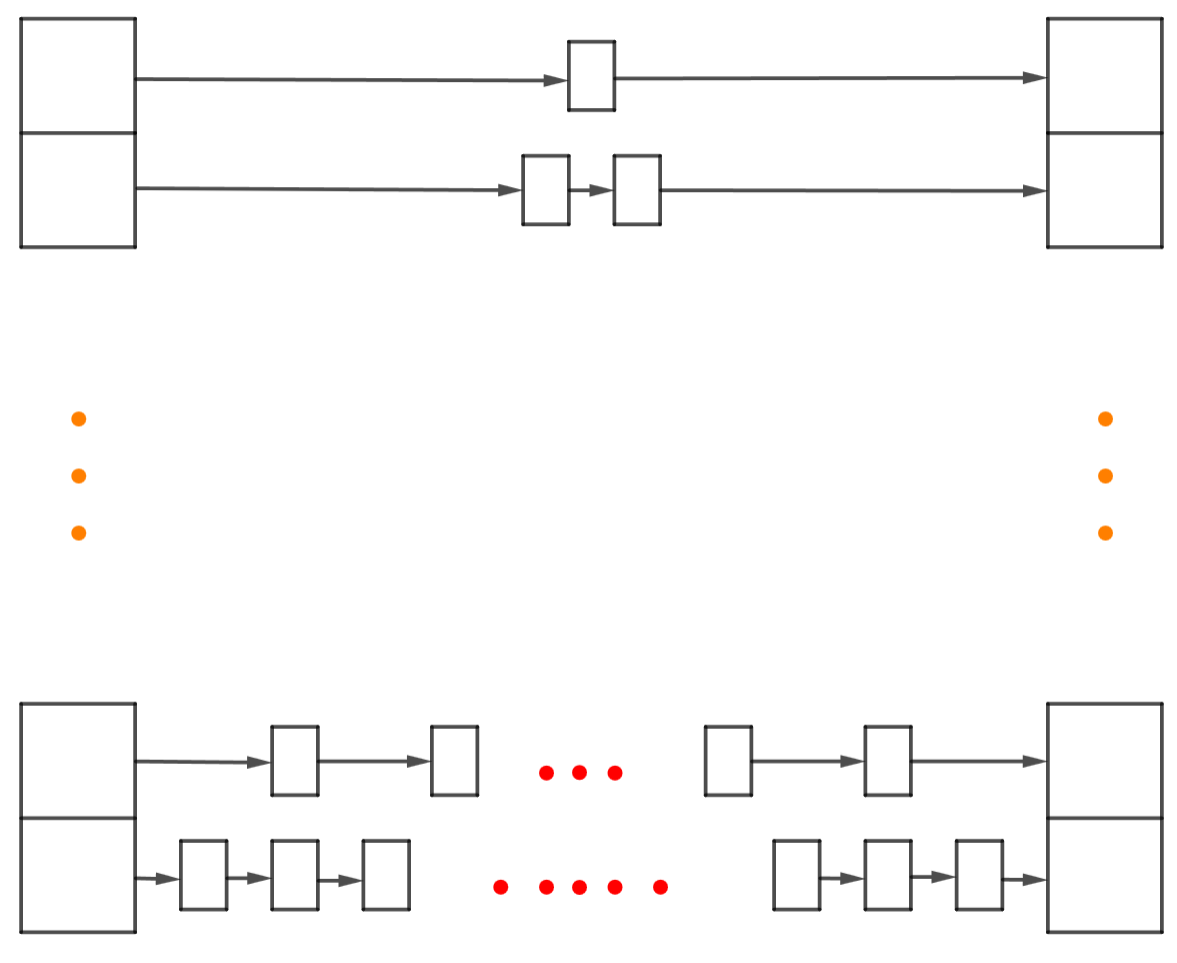
\includegraphics[scale=0.17]{./SL1.png}
  \end{center}
  estos valores tienen apuntadores para saber quién sigue en el orden, esto por cada posición en la lista original.
  Cómo es necesario mantener nuestros elementos ordenados y esto lo representamos por renglón (además de que eliminamos
  la mitad de los elementos en cada reglón de abajo hacia arriba), entonces nuestra construcción se toma
  $\mathcal{O}(n \log n)$. Además, anexaremos apuntadores de los elementos en niveles superiores a su nivel próximo inferior,
  a manera de que el elemento al que apunten sea el anterior más próximo en el orden, un bosquejo se vería de la
  siguiente manera
  \begin{center}
    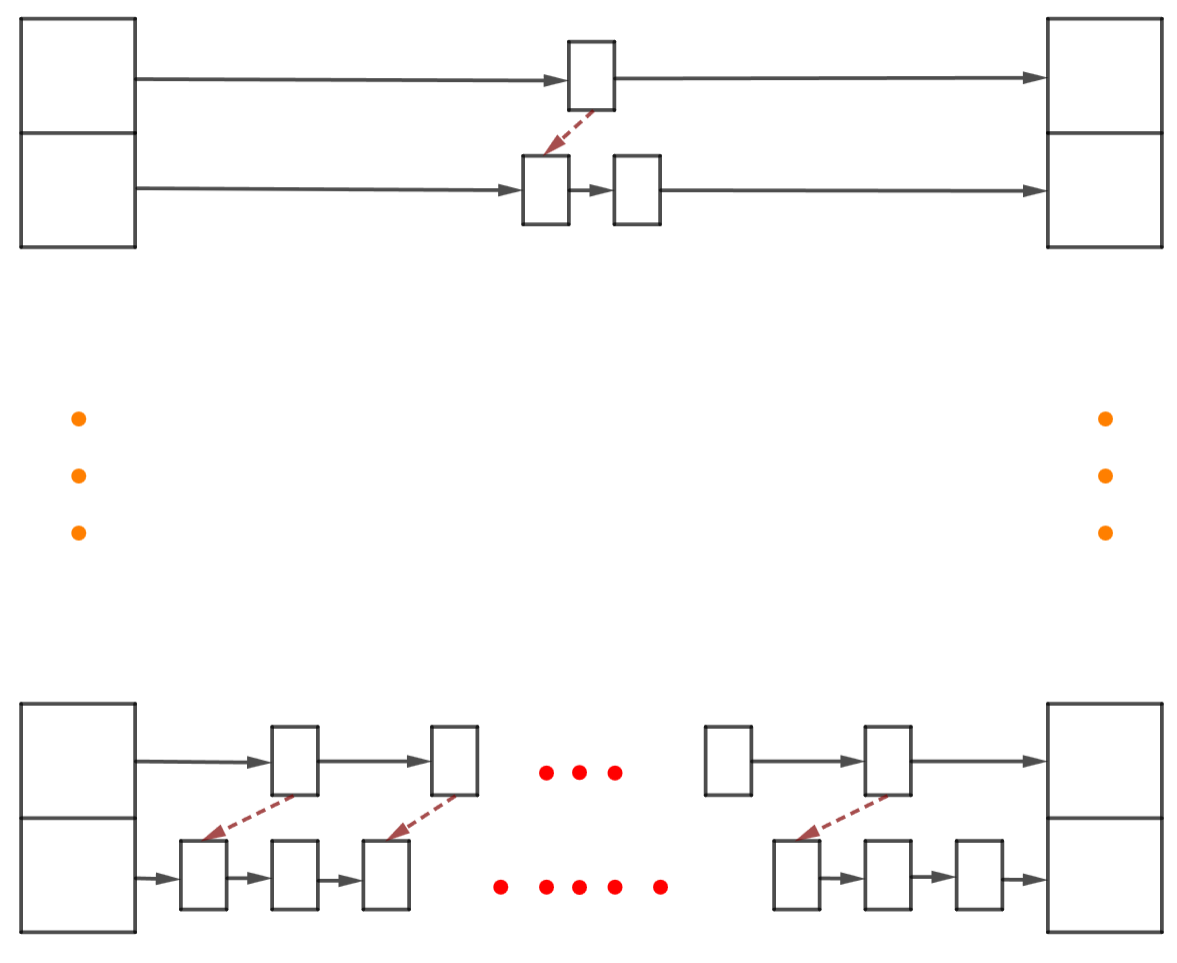
\includegraphics[scale=0.17]{./SL2.png}
  \end{center}
  notemos que esto último no nos $\mathcal{O}(n \log n)$. De la misma manera, cada nodo debe contener su respectivo índice
  suponiendo que tenemos una enumeración en el orden inicial (elementos del último nivel que están ordenado y se encuentran
  todos/completos).
\item \textbf{Insertar.} Cada vez que insertemos consultamos el número de inserciones hechas después de la
  construcción\footnote{Basta usar un contador.}, si este número es $o(n)$ respecto de los elementos originales
  entonces reconstruimos nuestra \textit{Skip-List}. Sino, entonces agregamos en el nivel 0 (de arriba hacia abajo)
  y apuntamos al anterior menor en el nivel inferior. Esto nos toma $\mathcal{O(\log n)}$ esperado (sólo cuándo
  está recién construida podemos garantizar esto), pues sólo realizamos una busqueda en el nivel 0 y en el 1 para
  encontrar su respectiva posición y apuntador.
\item \textbf{Consultar.} Debemos realizar una búsqueda desde el nivel 0, encontrar el último elemento menor al que búscamos
  consultar (o encontrar el elemento) e ir bajando por medio de sus apuntadores a sus niveles inferiores
  (de arriba hacia abajo). Esto hasta llegar al último nivel (puede que consultemos un elemento que no pertenece a $L$),
  lo que nos toma $\mathcal{O}(\log n)$ esperado.
\item \textbf{Borrar.} El borrado toma las mismas consideraciones que en el \textit{inserta} y utiliza el consulta para
  localizar el elemento y eliminar sus respectivas direcciones.
\end{enumerate}
Después de las indicaciones, observemos que
\begin{itemize}
\item[$a$)] Basta encontrar el índice del elemento en el nivel 0 y bajar en busca de su respectivo índice (esto
  gracias a que cada nodo contiene su índice y un apuntador al anterior. Esto nos toma $\mathcal{O}(\log n)$ esperado
  y sólo es exacto si $L$ no ha recibido modificaciones desde su creación.
\item[$b$)] De la misma manera que el inciso anterior, basta bajar hasta llegar al último valor mayor que $x$
  y observar su índice, digamos $i$, así sabemos que hay $i - 1$ elementos menor que $x$. Si llegamos al último
  nivel y todos los valores fueron mayores, significa que $x$ es menor respecto a los elementos de $L$ y devolvemos 0.
  Esto nos toma $\mathcal{O}(\log n)$ esperado.
\end{itemize}
  De lo anterior concluimos el ejercicio.
\hfill $\lhd$

%\subsection*{Respuesta}
%    <Tu respuesta aquí>

%\bigskip
